\subsubsection{Bioassay Development and Biopolymer Dynamics and Structure}
\index{Nau, Werner}

\paragraph{Research Team}
Werner Nau (Professor), Mara Florea (Graduate Student), Andreas Hennig (PhD Student), Apurba Koner (PhD Student), Roland Meyer (PhD Student), Harekrushna Sahoo (Ph.D. in November 2006, later Postdoc), Thomas Schwarzlose (Scientific Research Assistant), Hamdy El-Sheshtawy (PhD Student), Vanya Uzunova (Graduate Student), Roy D�Souza (Graduate Student) \\

Monitoring the rates by which enzymatic conversions occur is of
fundamental interest in biochemistry. In addition, pharmaceutical
industry is searching for potential inhibitors or activators of
enzymatic activity in the course of drug discovery. Among the most
sensitive and robust methods to monitor enzymatic reactions are
radioactive and fluorescence-based assays, among which the latter
are greatly desirable; in fact, fluorescence assays are gradually
substituting assays involving radiochemicals primarily in
industrial high-throughput screening (HTS), where frequently more
than 10000 compounds need to be tested daily, and where safety
issues and regulations remain a major concern. We are developing
novel fluorescence-based bioassays. In previous years, assays for
proteases and kinases, and for sensing antioxidant activity, were
developed, which were based on a genuine line of fluorescent
probes. These are known as fluorazophores, marketed as PuretimeTM
325 dyes, and they are characterized by an exceedingly long
fluorescence lifetime (up to 1 microsecond in water), which
allowed monitoring by a new nanosecond time-resolved detection
technique, for which we coined the name Nano-TRF (see publications
\cite{Nau5} and \cite{Nau13}). More recently, we have developed yet another
entirely new patent-pending assay principle, which will be
described below: supra-biomolecular tandem assays (see patent No.
1). In this new line of assays, macrocyclic host molecules are
being employed, which compete with enzymes for the substrate.


\paragraph{Highlights}

There is a substantial interest for biological assays, not only
for industrial HTS, but also laboratory microscale experiments in
biochemistry and biology, and screening and testing techniques for
medicinal diagnostics. Label-free assays, which allow the direct
monitoring of enzymatic activity with high sensitivity without
additional incubation steps at room temperature in homogeneous
solution, are most desirable, but extremely scarce. In 2006, we
have developed a new label-free enzyme assay type based on
unlabeled biological compounds along with supramolecular complexes
between a macrocyclic host and a fluorescent probe. The new assay
type is conceptually simple, but very versatile. As desired, it
operates in homogeneous solution, and allows direct monitoring by
fluorescence without the need for additional incubation steps or
chemical or analytical separations. These novel supra-biomolecular
tandem assays involve the addition of macrocyclic water-soluble
host molecules (e.g., cyclodextrins, calixarenes, cucurbiturils,
etc.) and water-soluble fluorescent dyes to a solution containing
active enzyme and substrate. In the course of the enzymatic
conversion, a change of fluorescence intensity and fluorescence
lifetime of the solution results, which can be employed to measure
enzyme kinetics, detect the activity of the enzyme, and monitor
the effect of potential inhibitors.

\begin{figure}[ht]
  \begin{center}
    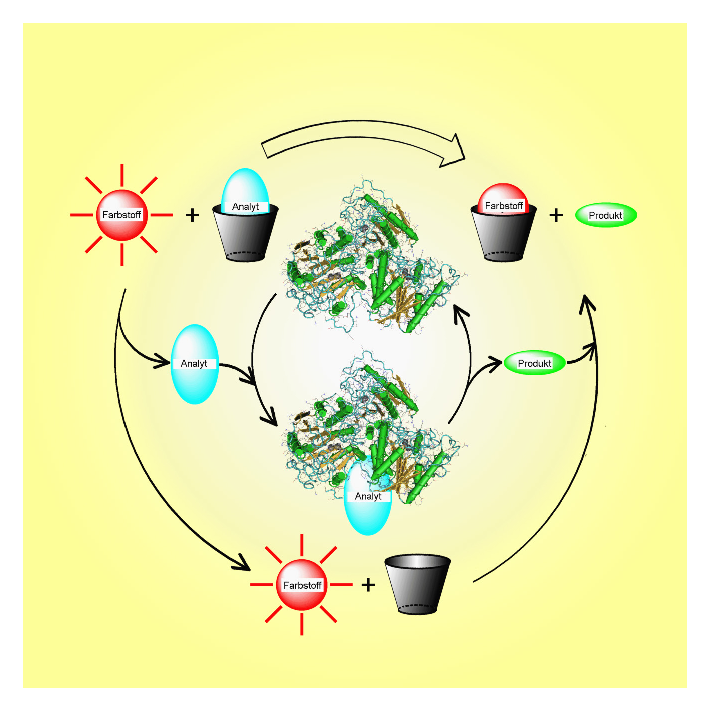
\includegraphics[width=\hsize]{Nau/Nau_2006_fig.pdf}
    \mycaption{ Working principle of an IN-OFF tandem assay.}\label{fig:nau-bild}
   \end{center}
\end{figure}

The method requires that (1)
the substrate and product of the reaction have a different
affinity to the macrocyclic host and (2) that the fluorescent
properties of the fluorescent dye differ in its complexed (by the
macrocycle) and uncomplexed forms. The former is expected whenever
the hydrophobic or electrostatic properties of substrate and
product differ significantly. For the latter effect (variations in
fluorescence properties of dyes upon complexation) numerous
examples are already available in the literature. The working
principle illustrated in Figure \ref{fig:nau-bild} is such that the substrate and
product displace the fluorescent dye to different degrees from the
macrocyclic host, and this differential displacement can be
translated into a change of its fluorescence. The latter can be
monitored with high sensitivity by established techniques. In our
laboratory, we perform steady-state fluorescence measurements on a
Varian Cary Eclipse spectrofluorometer and time-resolved
fluorescence measurements on a time-correlated single photon
counting set-up.\newline \newline Werner Nau is also involved in ``Supramolecular Functional Materials and Metalloenyzme Models''.


%Pictures are to be included via:



\myparagraph{Collaborations}
%
Bremen Area Collaborations:
\begin{enumerate}
\item {\sl International University Bremen} \\ Prof. K. Brix \\ Dye Stabilization in Live Cells
\\ Prof. A. Jeltsch \\ Investigation of Peptide Dynamics
\\ Prof. U. Kortz and Dr. M. Dickman \\ Structural Investigations
in Host-Guest Chemistry
\\ Prof. R. Richards \\Hybrid Materials
based on Cucurbiturils and Silver and Gold Nanoparticles
\\ Dr. D.
Roccatano \\ Study of the dynamics in solution of small peptides
by Molecular Dynamics simulation and time-resolved spectroscopic
techniques
 \\ Prof. S. Springer \\ Fluorescence spectroscopy of recombinant MHC class I molecules
 \\ Prof. M. Zacharias \\ Dynamics of end-to-end Contact Formation of Small Peptides
\end{enumerate}
National \& International Collaborations:
\begin{enumerate}
\item {\sl Hoffmann-La Roche Pharmaceuticals, Basel, Switzerland} \\ Dr. T. Enderle, Dr. D. Roth \\ Kinase Assays
\item {\sl Georgetown University, Washington DC, USA} \\ Prof. R. Weiss \\ Diffusion and Antioxidants in Polymer Films
\item {\sl Babha Atomic research Center, Mumbai, India} \\ Dr. J. Mohanty, Dr. Bhasikuttan, Dr. H. Pal \\ Supramolecular Photochemistry
\item {\sl Universidad Politecnica de Valencia} \\ Dr. U. Pischel \\ Supramolecular Sensors and Free Radical Reactions
\item {\sl Schlosspark-Klinik, Berlin} \\ Dr. Carl Erb \\ Messung von Antioxidantien im Kammerwasser und Blutplasma
\item {\sl Yarmouk University} \\ Prof. N. Saleh \\ Supramolecular Stabilization of Fungizides
\end{enumerate}


\paragraph{Grants}
\begin{enumerate}
\item Funded by private industry, Hoffmann-La
Roche/Pharmaceuticals, \emph{Novel Fast Time-resolved Assays
Allowing Rational Design of Fluorescent Substrates for Proteases
and Tyrosine, Serine, and Threonine Kinases}, (March 2004 -
February 2007) \item Funded by DAAD,  Grant with the Ac��es
Integradas Luso-Alemas/DAAD- GRICES Program
\emph{Cucurbituril-Based Lanthanide- Antenna Conjugates as Novel
Luminescent Supramolecular Devices}, (January 2005 - December
2008)
\end{enumerate}

\paragraph{Other Support Grants}
\begin{enumerate}


\item  {Egyptian governmental Ph.D. fellowship (4 years) for Hamdy El Sheshtawy (Egypt, since
November 2006) }

\item {DAAD Research fellowship for Prof. Na'il
Saleh (Jordan, summer 2006)}

\item  {DFG Travel Grant to attend the
First Joint International Symposium on Macrocyclic and
Supramolecular Chemistry, June 2006, Victoria, Canada}

\end{enumerate}
\paragraph{Honors and Awards}
%
\begin{enumerate}
\item Executive Member of the Photochemistry Section of the Gesellschaft Deutscher Chemiker GDCh
\item Elsevier Ph.D. Photoscientist Bursary 2006 (Ph.D. thesis of Dr. Huseyin Bakirci)
\end{enumerate}

\paragraph{Patents}
\begin{enumerate}
\item W. M. Nau, H. Bakirci, A. Hennig, ``Determination of
Concentration Changes'', German patent registration 10 2006 023083.3.
\end{enumerate}

\nocite{Nau1,Nau2,Nau3,Nau4,Nau5,Nau6,Nau7,Nau8,Nau9,Nau10,Nau11,Nau12,Nau13,Nau14,Nau15,Nau16}
